% Verweise lieber woanders?
Am Abend nach dem Versuch erhielten wir ausgedruckt alle Seismogramme, die mit Hammerschlag aufgenommenen direkt gestapelt. Daraus pickten wir die Ersteinsätze. Die gepickten Seismogramme sind dem Protokoll im Anhang angehängt. Die Seismogramme des Profils S11-S12 mit Hammerschlag wurden nicht gepickt, da diese Messung in diesem Protokoll nicht weiter ausgewertet wird.

\section{Profil S21-S22 }

Dieses Profil liegt über dem Basaltgang, was in Abbildung \ref{fig:Kartierung} mit der unterlegten Magnetik-Kartierung zu sehen ist. Das zugehörige Laufzeitdiagramm ist im Anhang beigefügt. Da unsere Fragestellung ist, ob sich diese Messmethode überhaupt für das Vermessen des Basaltgangs eignet, betrachten wir zunächst nur den Hinschuss. 
Wir vermuten, dass diese Schwankungen vom Basaltgang verursacht werden. Bei der Refraktionsseismik geht man von unendlichen geraden Platten aus. Wie wir in der Geoelektrik herausgefunden haben, ist der Basaltgang selbst stark verwittert und kann in keiner Weise als gerade Fläche angenommen werden.

\begin{figure}[!ht]
 \centering
 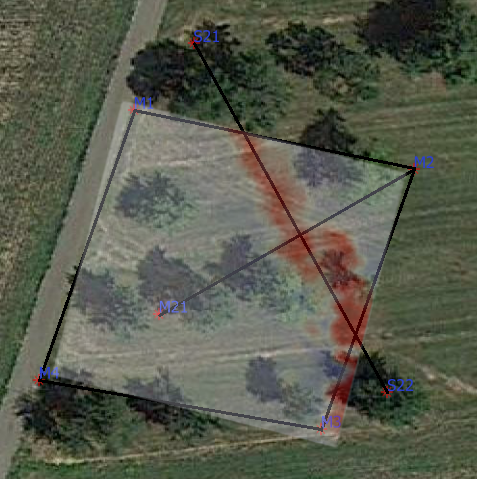
\includegraphics[width=0.5\textwidth]{fig/Seismik_kartierung}
 \caption[Profil S21-S22 mit untergelegter Magnetik-Kartierung]{Profil S21-S22 mit untergelegter Magnetik-Kartierung. Das Profil verläuft genau über dem Basaltgang. Die Grafik wurde von Katharina Adrion und Niels Gieseler übernommen.}
 \label{fig:Kartierung}
\end{figure}

Wie in Kapitel \ref{sec:zweiSchichten} beschrieben wurde, werden nun die seismischen Geschwindigkeiten, die relevanten Winkel und die Schichtmächtigkeiten bestimmt.\\
Die Rechnungen wurden mit Python durchgeführt und die Ergebnisse sind in Tabelle \ref{tab:S21-S22} aufgeführt.\\

% Die Geschwindigkeiten 
% \begin{align}
%  v_1 &= \SI{181.82}{m/s} \\
%  v_2 &= \SI{615.38}{m/s} \\
%  v_3 &= \SI{1818.18}{m/s}
% \end{align}
% werden aus den Geradensteigungen bestimmt.
% Daraus werden die Winkel 
% \begin{align}
%  \vartheta_1 &= \SI{0.2999}{rad} \\
%  \vartheta_2 &= \SI{0.3453}{rad} \\
%  \vartheta_12 &= \SI{0.1002}{rad}
% \end{align}
% berechnet.
Die Schichtmächtigkeit der ersten Schicht ist $d_1 =\SI{0.95}{m}$ und für die Schichtmächtigkeit der zweiten Schicht ergibt sich $d2 = \SI{2.50}{m}$.\\

Für die Fehlerbetrachtung haben wir neue, etwas abweichende aber plausible , 
Ausgleichsgeraden durch die Messpunkte gelegt. Mit den neuen Werten wird die Berechnung wiederholt. Die Differenz der neuen Größen und zuvor berechneten optimalen Größen ist der Fehler auf die Werte. In Tabelle \ref{tab:S21-S22} werden die Werte, die bereits berechnet wurden, als Optimalwerte bezeichnet. Als Toleranzwerte bezeichnen wir die Werte die aus den weniger passenden Fitgeraden berechnet wurden. Der Fehler ist die Differenz zwischen diesen beiden Messungen.

%%%%%%%%%%%%%%%%%%%%%%%%%%%%%%%%%%%%

\begin{table}[!ht]
\centering
\caption{Werte der Profilmessung S21-S22}
\label{tab:S21-S22}
\begin{tabular}{lllllll}
\toprule
Größe   & Optimalwert   & Toleranzwert   & Fehler \\
\midrule
$v_1$ in m/s & 181.82 & 214.29 & 32.47 \\
$v_2$ in m/s & 615.38 & 754.72 & 139.34 \\
$v_3$ in m/s & 1818.18 & 1858.41 & 40.23 \\
$\vartheta_1$ in rad & 0.2999 & 0.2879 & 0.0100 \\
$\vartheta_2$ in rad & 0.3453 & 0.4182 & 0.0732 \\
$\vartheta_{12}$ in rad & 0.1002 & 0.1156 & 0.0154 \\
$d_1$ in m & 0.95 & 1.15 & 0.20 \\
$d_2$ in m & 2.50 & 2.64 & 0.14 \\

\bottomrule
\end{tabular}
\end{table}

%%%%%%%%%%%%%%%%%%%%%%%%%%%%%%%%%%%%%%

Die Schichtgrenze in $\SI{0.95 \pm 0.20}{m}$  Tiefe deutet darauf hin, dass hier der Basaltgang anfängt. Allerdings haben wir in $\SI{2.50 \pm 0.14}{m}$ Tiefe schon die nächste Schichtgrenze. Leider passen die berechneten Geschwindigkeiten nicht zu den seismischen Geschwindigkeiten von Basalt. Die Seismische Geschwindigkeit von Basalt sind $\SI{4000}{m/s}$ und unsere höchste gemessene Geschwindigkeit ist $\SI{1818.18 \pm 40.23}{m/s}$.\\
Die Refraktionsseismik eignet sich wie vermutet wahrscheinlich einfach nicht zum bestimmen der Tiefe des Basaltgangs. 


\section{Profil S31-S32}

Das Laufzeitdiagramm (siehe Anhang) mit eingetragenem Hin- und Rückschuss dieses Profils ist achsensymmetrisch um $x=20$\,m. Daraus lässt sich schließen, dass keine geneigten Schichtgrenzen vorliegen.
Diese Messung wurde durchgeführt, um einen Vergleich zum Profil S21-S22 zu haben.
Wie bereits für das Profil Profil S21-S22 wurden die in Tabelle \ref{tab:S31-S32} eingetragenen Werte berechnet. Als Fehler ist die Differenz des Toleranzwertes und des Optimalwertes eingetragen.\\


%%%%%%%%%%%%%%%%%%%%%%%%%%%%%%%%%%%%

\begin{table}[!ht]
\centering
\caption{Werte der Profilmessung S31-S32}
\label{tab:S31-S32}
\begin{tabular}{lllllll}
\toprule
Größe   & Optimalwert   & Toleranzwert   & Fehler \\
\midrule
$v_1$ in m/s & 114.29 & 240.00 &  125.71\\
$v_2$ in m/s & 824.74 & 1030.93 & 206.19 \\
$v_3$ in m/s & 2210.53 & 2270.27 & 59.26 \\
$\vartheta_1$ in rad & 0.139 & 0.235 & 0.096  \\
$\vartheta_2$ in rad & 0.382 & 0.471 & 0.089 \\
$\vartheta_{12}$ in rad & 0.052 & 0.106 & 0.054 \\
$d_1$ in m & 0.49 & 1.05 & 0.56 \\
$d_2$ in m & 3.08 & 3.93 & 0.85 \\

\bottomrule
\end{tabular}
\end{table}

%%%%%%%%%%%%%%%%%%%%%%%%%%%%%%%%%%%%%%




Die Fehler sind teilweise leider sehr hoch, was aber daran liegt, dass das Laufzeitdiagramm sehr viel Spielraum für die Lage der Geraden lies. 
Wir können hier aber zwei Schichtgrenzen bestimmen, die bei Berücksichtigung der Fehler, in der gleichen Tiefe liegen, wie die Schichtgrenzen des Profils S21-S22. Es handelt sich also vermutlich um die gleichen gemessenen Schichten.

\section{Vergleich Profil S21-S22 und Profil S31-S32}

Aus der Magnetik und Geoelektrik wissen wir, dass unter dem Profil S31-S32 kein Basaltgang ist. Daher können wir nun mit großer Sicherheit sagen, dass die berechneten Schichtengrenzen nicht die die Obergrenze des Basalts ist. Somit eignet sich die Refraktionsseismik eindeutig nicht zur Bestimmung der Lage des Basaltgangs. Vergleicht man das Diagramm der Messung über und neben dem Basaltgang, stellt man fest, dass die Werte des Profils S31-S32 wesentlich weniger Schwankungen haben als die des Profils S21-S22.

\section{Profil S11-S12}

Das Laufzeitdiagramm der Messung am Profil S11-S12 mit S.I.S.Sy befindet sich in Abbildung \ref{fig:plotsissy}. Sowohl beim Hin- als auch beim Rückschuss sind zwei gerade Abschnitte zu erkennen. Beim Rückschuss weichen die gemessenen Werte im Bereich der Profilkoordinate 50\,m bis 95\,m relativ stark von der Geradenform ab. Dies könnte an der oberflächlich in diesem Bereich stark ausgeprägten Topographie liegen. Beim Hinschuss ist dies jedoch nicht so deutlich im Laufzeitdiagramm zu sehen. Zunächst wurden für die Auswertung die Schichtdicke für Hin-und Rückschuss mit der Annahme nicht geneigter Schichtgrenzen berechnet. Da diese Werte 1,3\,m Differenz aufwiesen, wurde eine geneigte Schicht über dem homogenen Halbraum angenommen.

\begin{figure}[!ht]
 \centering
 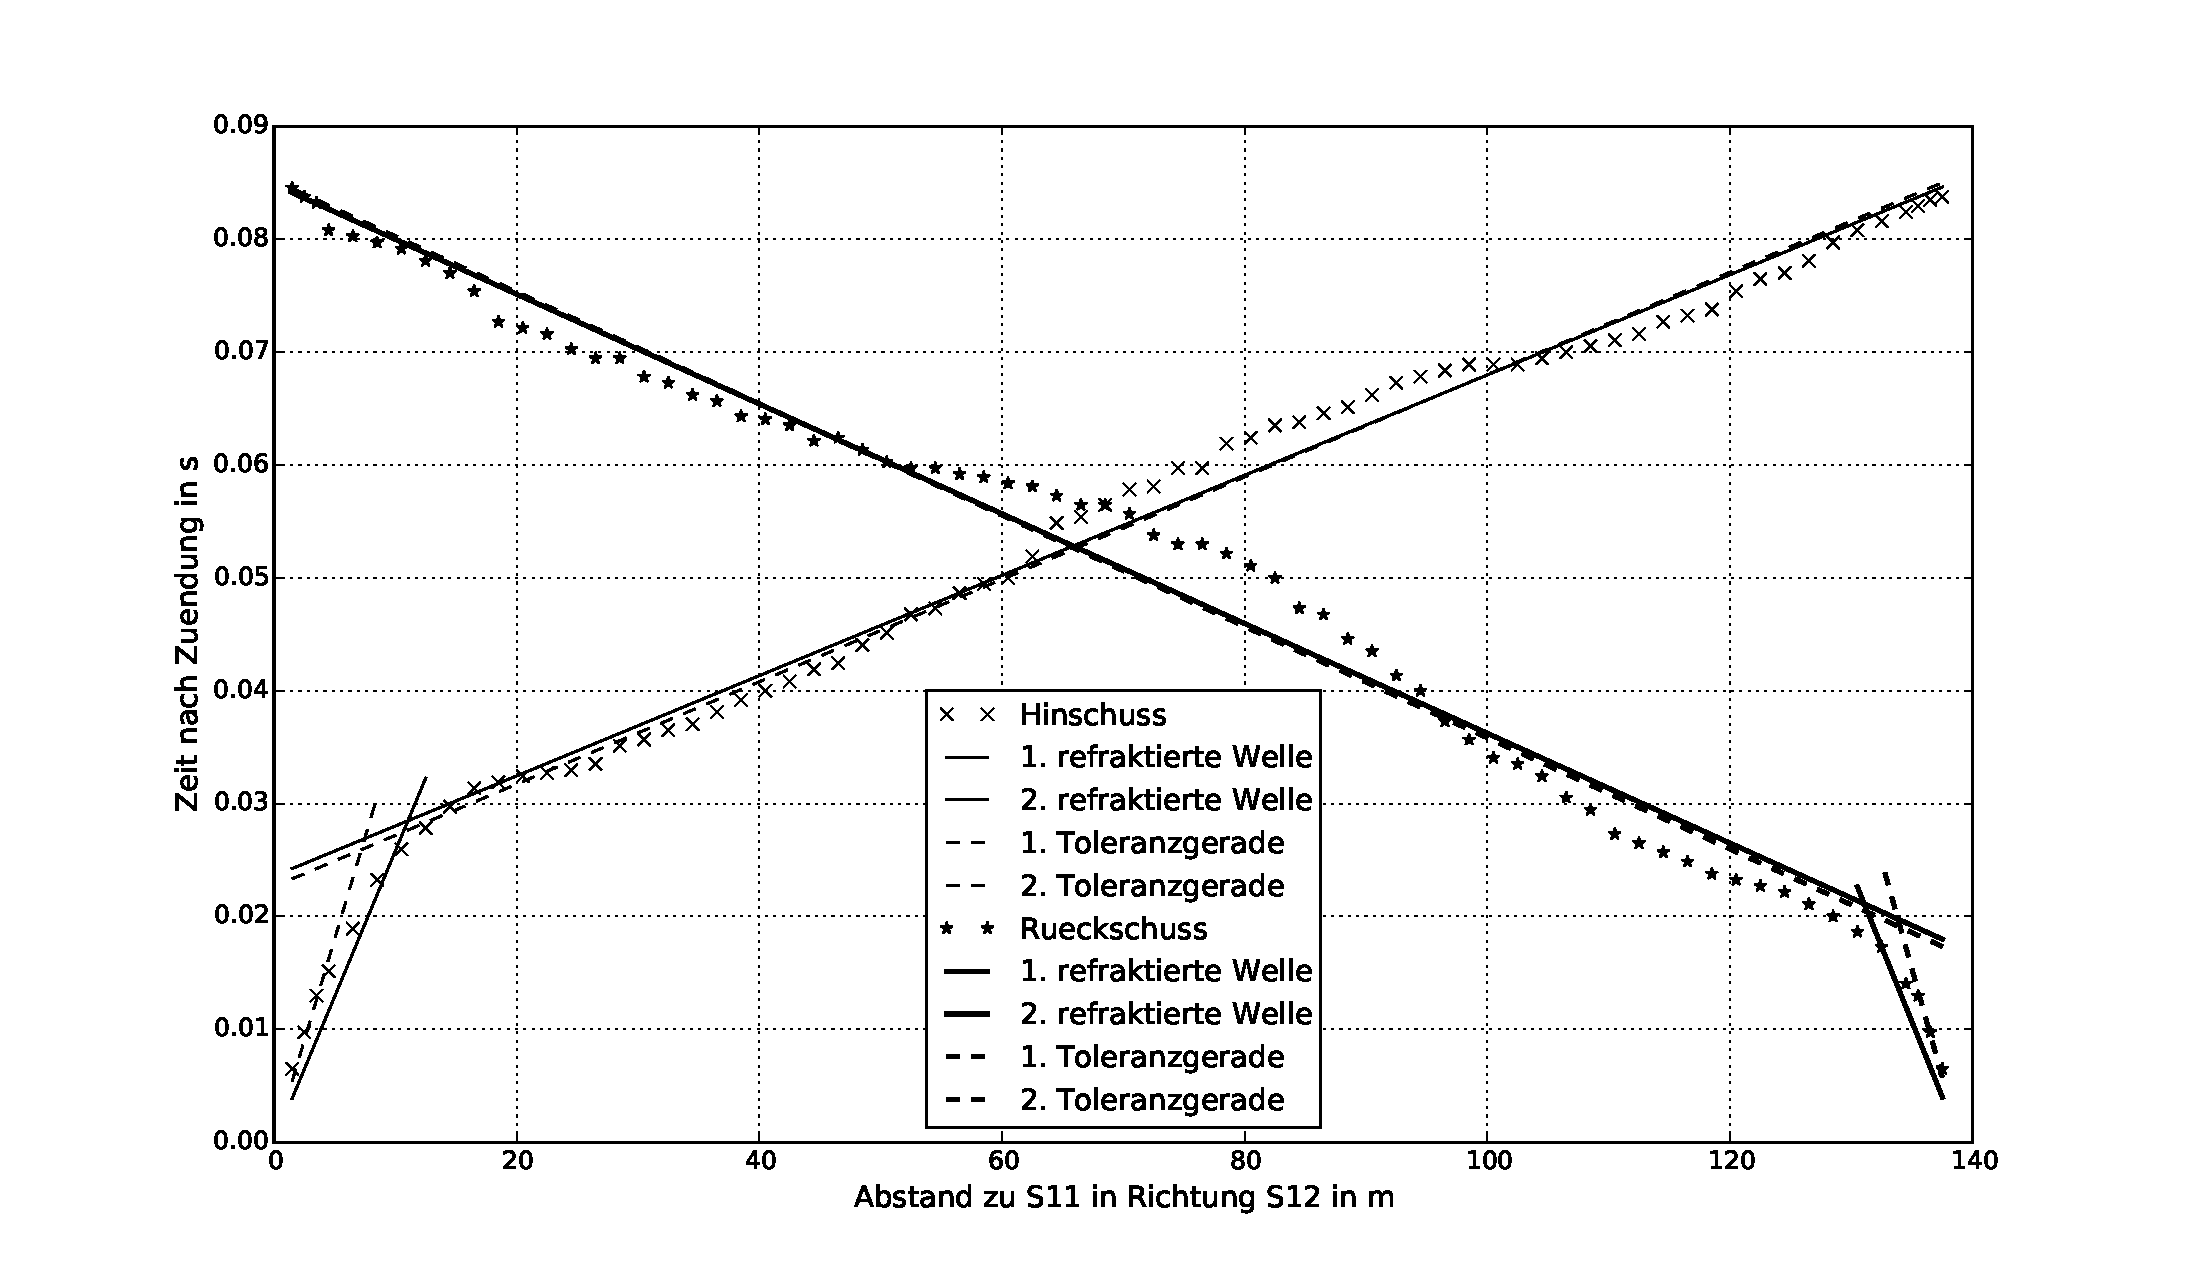
\includegraphics[width=\textwidth]{fig/plotsissy}
 \caption{Laufzeit und gefittete Geraden der Messung mit S.I.S.Sy auf Profil S11-S12}
 \label{fig:plotsissy}
\end{figure}

Die Berechnung der in Tabelle \ref{tab:werte} aufgeführten Werte wurde wie in Kapitel \ref{sec:geneigteSchicht} beschrieben durchgeführt. Da die Intercept-Zeit des Hinschusses größer als die des Rückschusses ist, beziehen sich die Werte mit Index $+$ auf den Hinschuss und die mit Index $-$ auf den Rückschuss. Als Toleranzwerte werden wieder diejenigen Werte bezeichnet, die mit einer anderen Wahl der Geraden berechnet wurden und dennoch im optischen Toleranzbereich liegen. Die Differenz dieses Werts und des Werts der per Augenmaß am bestem passenden Geraden ergibt dann den Fehler der jeweiligen Größe. Da beim Hin- und Rückschuss nicht genau dieselbe Geschwindigkeit der direkten Welle bestimmt wurde, wird der Mittelwert $v_1$ dieser beiden Geschwindigkeiten für die weiteren Berechnungen verwendet. Vergleicht man die Werte für $d_-$ und $d_+-s\sin(\alpha)$, weichen sie 0,08\,m voneinander ab. Sie stimmen nicht genau überein, weil die Geschwindigkeit $v_1$ der direkten Welle aus den Werten von Hin- und Rückschuss gemittelt wurde. Die Richtigkeit Rechnung kann dadurch aber bestätigt werden.

\begin{table}[!ht]
\centering
\caption{Werte der Profilmessung S11-S12}
\label{tab:werte}
\begin{tabular}{llrrr}
\toprule
Größe & Einheit & Optimalwert   & Toleranzwert   & Fehler \\
\midrule
$t_{i+}$ & s & 0.02357  &0.02265 & 0.00092\\
$t_{i-}$ &s & 0.01725  &0.01659 & 0.00066\\
$\q{v}{1\,hin}$ & m/s &387.68 & 277.84&109.85\\
$\q{v}{1\,rueck}$ & m/s & 375.92& 261.14&114.78\\
$v_1$ & m/s & 381.80 & 269.49& 112.31\\
$v_{2+}$ & m/s & 2251.38  &2204.01 & 47.37\\
$v_{2-}$ & m/s & 2055.70 &2027.08 & 28.61\\
$v_2$ & m/s & 2149.02 &2111.82 & 37.20\\
$\vartheta$ & $^\circ$ & 10.23 & 7.33& 2.90\\
$\alpha$ & $^\circ$ & 0.47 & 0.31& 0.16\\
$d_+$ & m & 4.57 & 3.08& 1.50\\
$d_-$ & m & 3.35 &2.25 & 1.09\\
$d_+-s\sin(\alpha)$ & m & 3.43 & 2.33& -\\
$s$&m&139&-&-\\
\bottomrule
\end{tabular}
\end{table}

% \begin{figure}[!ht]
%  \centering
%  \includegraphics[width=\textwidth]{fig/}
%  \caption{}
%  \label{fig:}
% \end{figure}
Zusammenfassung


Die Messung auf dem Profril S11-S12, die mit S.I.S.Sy durchgeführt wurde, liefert sehr gute Ergebnisse. Unsere Fragestellung war, in erster Linie der Verlgeich dieser Messmethode mit der Geoelektrik. In der Geoelektrik hat man viel Interpretationsfreiraum die Anzahl und die Tiefe von Schichten angeht. Die Seismik liefert eindeutigere Ergebnisse. So sind wir uns sehr sicher, das wir genau eine Schichtgreneze in einer Tiefe von $d_+= \SI{4,57 \pm 1,50}{m}$, bzw. $d_-= \SI{3,35 \pm 1,09}{m}$, haben. Die Schicht ist geneigt, weshalb es auch Schichttiefen gibt, eine Amanfang, die zweite am Ende des Profils. In der Geoelektrik wurde in einem der berechneten Modelle ebenfalls eine Schichtgrenze in etwa dieser Tiefe gefunden. Ändern sich die seismischen und geoelektrischen Eigenschaften gleichzeitig, kann es sich um die gleiche Schicht handeln. \\
Optimal wäre es für die Messung gewesen, wenn wir ein ebenes Profil verwendet hätten. Wir haben ein Profil gesucht mit möglciht wenig Topographie, eine kleinere Erhebung haben wir aber leider trotzdem auf dem Messprofil. Dieser Hügel ist vermutlich in als Kurve in den Laufzeitdiagramme zu erkennen.\\
Trotzdem können wir sagen, dass sich die Seismik gut zum untersuchen des Untergrunds auf Profil S11-S12 eignet. \\
Anders verhält es sich beim Versuch den Basaltgang mit der Hammerschlag-Methode nachzuweisen. 
